\documentclass[12pt]{article}


\usepackage{afterpage}
\usepackage[usenames,dvipsnames]{xcolor}
\usepackage{graphicx}
\usepackage{hyperref}


\title{\textbf{{\color{white}Informe Azul}}}
\author{{\color{white}Alejandra Monz\'on C312}\\ {\color{white}Mari\'e del Valle C311}}
\date{}

\begin{document}
	\maketitle
	\pagecolor{RoyalBlue}\afterpage{\nopagecolor}
	
	\newpage
	    
    \section*{Din\'amica del juego}
    El juego comienza en la regla \texttt{new\_game(N)}, donde \texttt{N} son la cantidad de jugadores que participan en el juego.
    
	En la simulaci\'on del juego se destacan dos hechos que almacenan los estados del juego y de los jugadores. Dichos hechos son \texttt{\textbf{game\_state}(N,Bag,Factories,
	Center,Stack,InitialPlayer,CurrentPlayer,State)} y \texttt{\textbf{player\_state}(Player,
	Wall,Pattern,Floor,Score)} respectivamente. 
	
	La simulaci\'on comienza inicializando la bolsa y las f\'abricas con los azulejos y los jugadores, con el muro, patr\'on y piso creados. Los azulejos que se ponen en las f\'abricas se eligen aleatoriamente y se eliminan de la bolsa. Adem\'as se elige aleatoriamente un jugador inicial, que comienza la \texttt{fase\_1}. 
	
	El objetivo es, una vez iniciado el juego con \texttt{State = inicialized}, buscar si existe una secuencia de estados (\texttt{game\_state})\ref{move} que permitan alcanzar el \texttt{State = win}, pasando por diferentes estados como  \texttt{State = \{fase\_1, fase\_2, fase\_3, over\}}.
	
		\begin{figure}[h]
		\begin{center}
			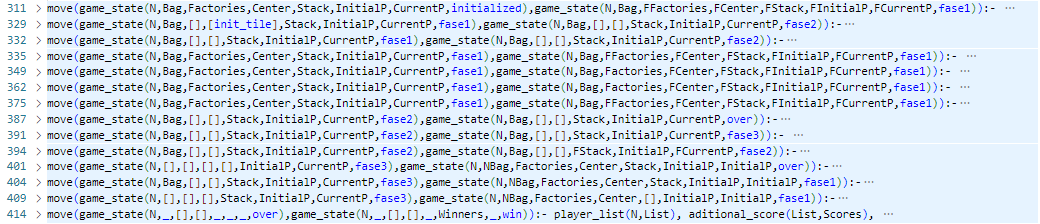
\includegraphics[scale=0.6]{../move}
			\label{move}
		\end{center}
	\end{figure}	
		
	
	\subsection*{Fase 1}
	En esta fase, el jugador inicial, empieza el juego, eligiendo robar de una f\'abrica; luego contin\'ua el juego con el siguiente jugador, el cual se define como el hecho \texttt{next\_player(CurrentPlayer,NumberOfPlayers,NextPlayer)}.
	\begin{figure}[h]
		\begin{center}
			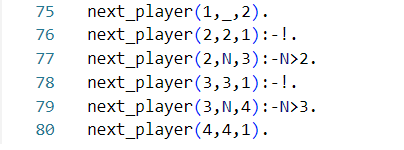
\includegraphics[scale=1.0]{../nextplayer}
		\end{center}
	\end{figure}

     En el centro se encontrar\'a la ficha inicial(\texttt{init\_tile}), hasta que alg\'un jugador decida robar azulejos del centro, design\'andose a s\'i mismo el pr\'oximo jugador inicial de la futura \texttt{fase\_1}.
	
	\subsection*{M\'etodo de elegir jugada}
	El m\'etodo \texttt{best\_move} consistir\'ia en lo siguiente:
	
	Cada jugador en dependencia del estado de su tablero (patr\'on, muro), tiene un conjunto de jugadas factibles seg\'un los azulejos disponibles en las f\'abricas y el centro. Estas jugadas se definen como v\'alidas o factibles, si cumplen que para un color \textit{\textbf{x}} de azulejos, en una fila \textit{\textbf{r}} del patr\'on, no se ha puesto en la fila \textit{\textbf{r}} del muro azulejo de color \textit{\textbf{x}} y en la fila \textit{\textbf{r}} del patr\'on no se ha puesto azulejo de color distinto de \textit{\textbf{x}}. Esto se verifica en la siguiente regla:
	\begin{figure}[h]
		\begin{center}
			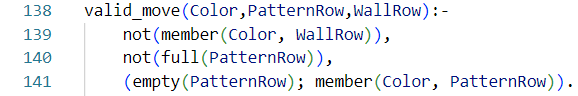
\includegraphics[scale=1.0]{../validmove}
		\end{center}
	\end{figure}
    
    A partir de dichas jugadas factibles, se seleccionan las mejores jugadas por f\'abricas y centro, atendiendo a un evaluaci\'on golosa que se le asigna a cada jugada. La siguente regla se define como \texttt{evaluate(Color,ZeroList,Floor,Evaluation,
    	BonnusPoints)}.
    
	\begin{figure}[h]
		\begin{center}
			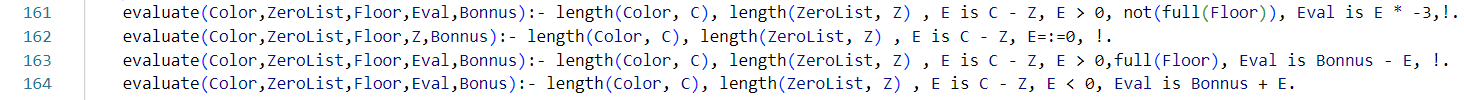
\includegraphics[scale=0.5]{../evaluate_}
		\end{center}
	\end{figure}
    
    Esta regla se divide en varios casos:
    \begin{itemize}
    	\item[1.] La cantidad azulejos de color \texttt{Color}, es mayor que la cantidad de espacios disponibles en la fila del patr\'on y el piso no est\'a lleno, por lo que se restar\'ian puntos al jugador por los azulejos sobrantes que se pondr\'ian en el suelo. Por ello, se penaliza con -3 puntos por cada azulejos que sobre.    	
    	\item[2.] La cantidad de azulejos de color \texttt{Color}, es igual a la cantidad de espacios vaci\'os en la fila del patr\'on disponible, por lo que se asigna, como evaluaci\'on, la cantidad de espacios vac\'ios que se llenar\'an con los azulejos.    	
    	\item [3.] La cantidad de azulejos de color \texttt{Color}, es mayor que los espacios disponibles en la fila del patr\'on y el suelo est\'a lleno, por tanto no se pierden puntos por los azulejos sobrantes y se completar\'ia la fila. La evaluaci\'on de estas jugadas es igual a la cantidad de azulejos en la fila, menos la cantidad de azulejos que se descartar\'ian.
    	\item [4.] La cantidad de azulejos de color \texttt{Color}, es menor que los espacios disponibles en la fila del patr\'on. En este caso se penalizar\'ia por los espacios que quedan disponibles, luego de poner los azulejos.   	

    \end{itemize}
    
  Importante destacar que poner los azulejos directamente en el suelo es una jugada v\'alida y que en caso de que el suelo este lleno, esos azulejos ir\'ian directo a la tapa de la caja.
  
  Luego de elegir una mejor jugada por f\'abricas y centro, se selecciona la mejor de ellas y se ejecuta esta, actualizando el patr\'on y/o el suelo del jugador, as\'i como la tapa de la caja, en algunos casos.
  
  \begin{figure}[h]
  	\begin{center}
  		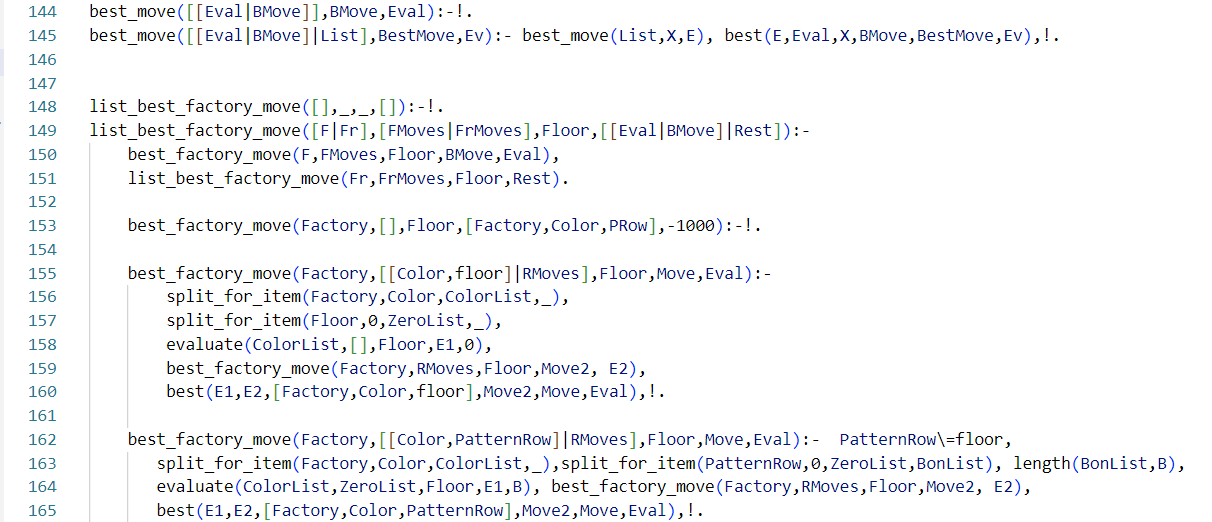
\includegraphics[scale=0.6]{../bestmove}  		
  	  	\end{center}
  \end{figure} 

\subsubsection*{Condici\'on de Parada}  
	La \texttt{fase\_1} finaliza cuando no queden azulejos disponibles en las f\'abricas y en el centro.
	
	\subsection*{Fase 2}
	En esta fase, se actualiza el muro de los jugadores, poniendo en ellos los azulejos correspondientes a las filas llenas de los patrones y se actualiza la puntuaci\'on de los jugadores.
		
	\subsubsection*{M\'etodo para poner azulejos en Muro}
	La acci\'on de actualizar el patr\'on se define como una revisi\'on de cada fila de el patr\'on en busca de una llena de azulejos, para trasladar un ejemplar de dicha fila hacia el muro y los restantes hacia la tapa de la caja.
	
	Una vez puesto el azulejo en el muro, se realiza el conteo de los puntos que se deben adicionar al jugador.
	
	La regla  \texttt{cover\_wall} realiza el procedimiento anteriormente descrito.
	
	\begin{figure}[h]
		\begin{center}
			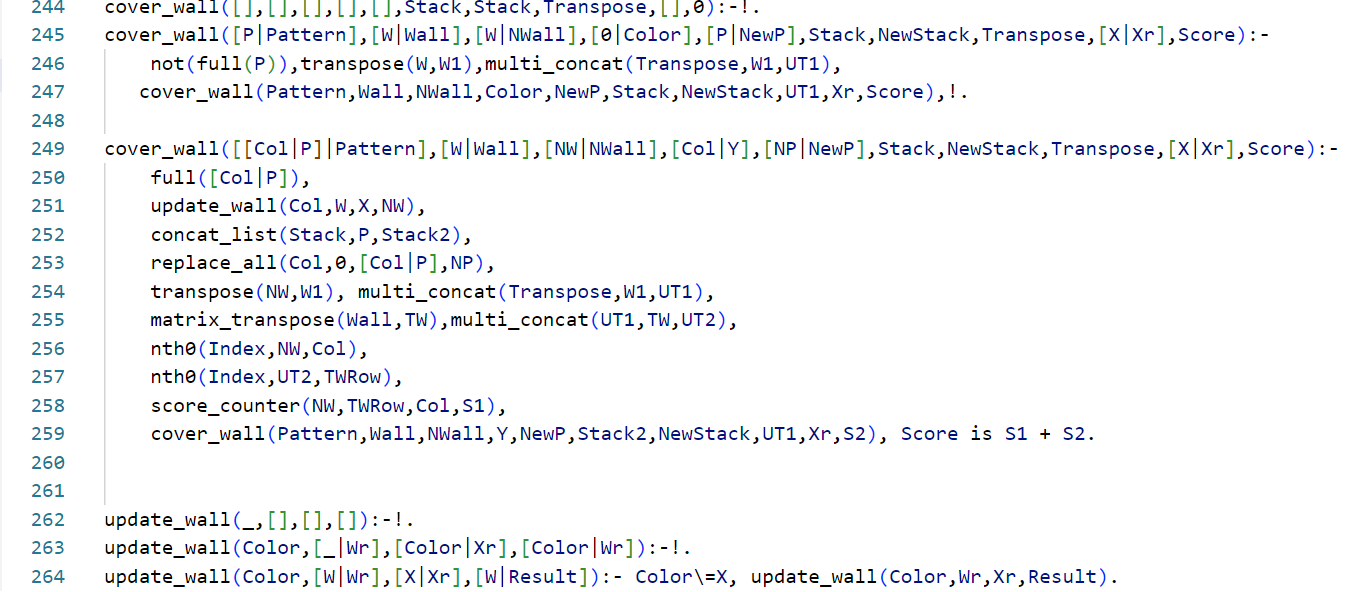
\includegraphics[scale=0.7]{../coverWall}  		
		\end{center}
	\end{figure} 

\begin{figure}[h]
	\begin{center}
		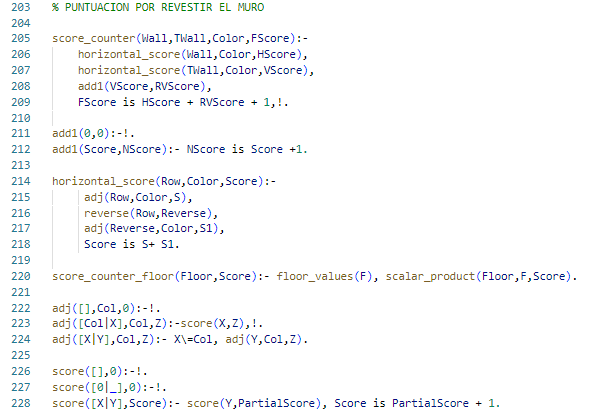
\includegraphics[scale=0.8]{../puntuacion}  		
	\end{center}
\end{figure} 
Cada vez que se traslada un azulejos de una fila del patr\'on a la fila correspondiente del muro, se verifica la adyacencia horizontal y vertical con otros azulejos para saber en cuanto incrementar la puntiaci\'on del jugador. 

Adem\'as, antes de actualizar el muro y puntuaci\'on del siguiente jugador, se restan los puntos correspondientes a los azulejos en el suelo del jugador y pasar estos a la tapa de la caja. Si entre dichos azulejos se encuentra la ficha inicial, pasar esta al centro.
	
	\newpage
	\subsubsection*{Condici\'on de parada}
	La \texttt{fase\_2} termina en dos posibles casos:
	\begin{itemize}
		\item [1.] Se termina de actualizar muro de todos los jugadores y ninguno completo una fila de dicho muro, por lo que se pasa a \texttt{fase\_3}.
		\item [2.] Al analizar a todos los jugadores, al menos uno tiene al menos una fila completa de azulejos, con lo cual se pasa al estado \texttt{over} del juego.
		
	\end{itemize}
	\subsection*{Fase 3}
	En la \texttt{fase\_3}, se inicializan con azulejos de la bolsa las f\'abricas y se verifica que en el centro se encuentre la ficha inicial. En el caso que la bolsa est\'e vac\'ia se pasan los azulejos de la tapa de la caja a la bolsa para proceder al llenado de las f\'abricas.
	
	\subsubsection*{Condici\'on de parada}
	Tiene dos condiciones de parada:
	\begin{itemize}
		\item [1.] Si hay azulejos en bolsa o en la tapa de la caja se llenan cuantas f\'abricas sean posible y se pasa a \texttt{fase\_1} 
		\item [2.] En caso contrario, no quedan m\'as jugadas posibles a realizar por los jugadores, ya que no hay azulejos en las f\'abricas, por lo que se pasa al estado \texttt{over} del juego.	
		
	\end{itemize}

\subsection*{Estado Over}
Aqu\'i, como se termina el juego, se agrega a cada jugador los puntos adicionales por completar fila, columna o color de azulejo. Adem\'as se selecciona \'el(los) ganador(es), atendiendo a la mayor cantidad de puntos y en caso de empate a la mayor cantidad de filas completadas. De este estado se pasa directamente al estado \texttt{win}, el cual dar\'a por terminada la simulaci\'on del juego.
	
	
\end{document}